% fig for 1D slice of plasma
\begin{figure}[!b]
\vspace{-1.5em}
\centering
\subcaptionbox{\emph{by bit plane}
(\sbit)}{{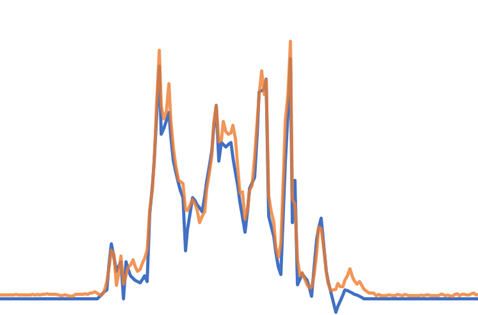
\includegraphics[width=0.48\linewidth]{gradient/1d_plasma_by_bit_plane}\vspace{-0.5em}}}
\subcaptionbox{\emph{by wavelet norm}
(\swav)}{{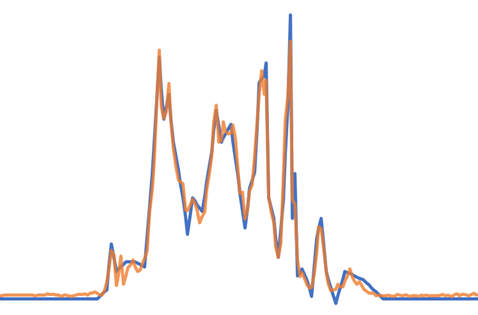
\includegraphics[width=0.48\linewidth]{gradient/1d_plasma_by_wavelet_norm}\vspace{-0.5em}}}
\vspace{-0.5em}
\caption{A 1D line extracted from \emph{plasma}, and reconstructed using \sbit and \swav at 0.6 bps.
The original data is in orange and the reconstructions are in blue. \sbit is worse at capturing the
function values (seen as a slight vertical shift) but it is comparable to \swav in capturing the
shape of the function, which is important for gradient computation.}
\label{fig:bit-plane-vs-wavelet-norm-gradient}
\vspace{-1em}
\end{figure}

% figure for gradient error
\begin{figure*}[t]
\centering
\subcaptionbox{\emph{boiler}, $[2.020e{-}9, 0.148]$}{%
{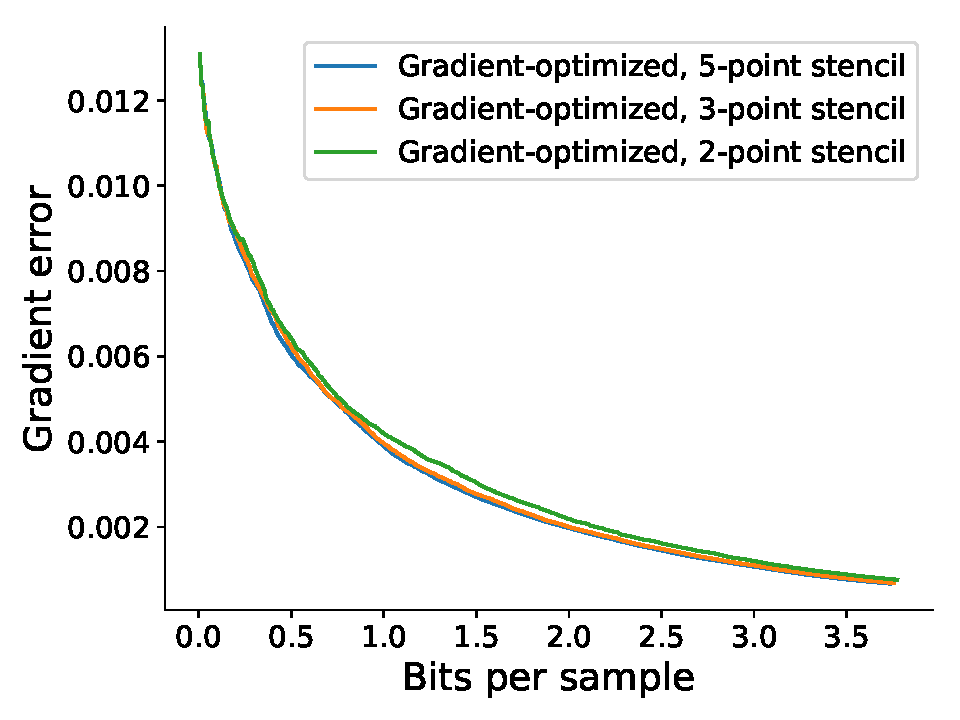
\includegraphics[width=0.24\linewidth]{gradient/gradient-optimized-boiler}\vspace{-0.5em}}}
\subcaptionbox{\emph{diffusivity} $[1.063e {-}10, 0.497]$}{%
{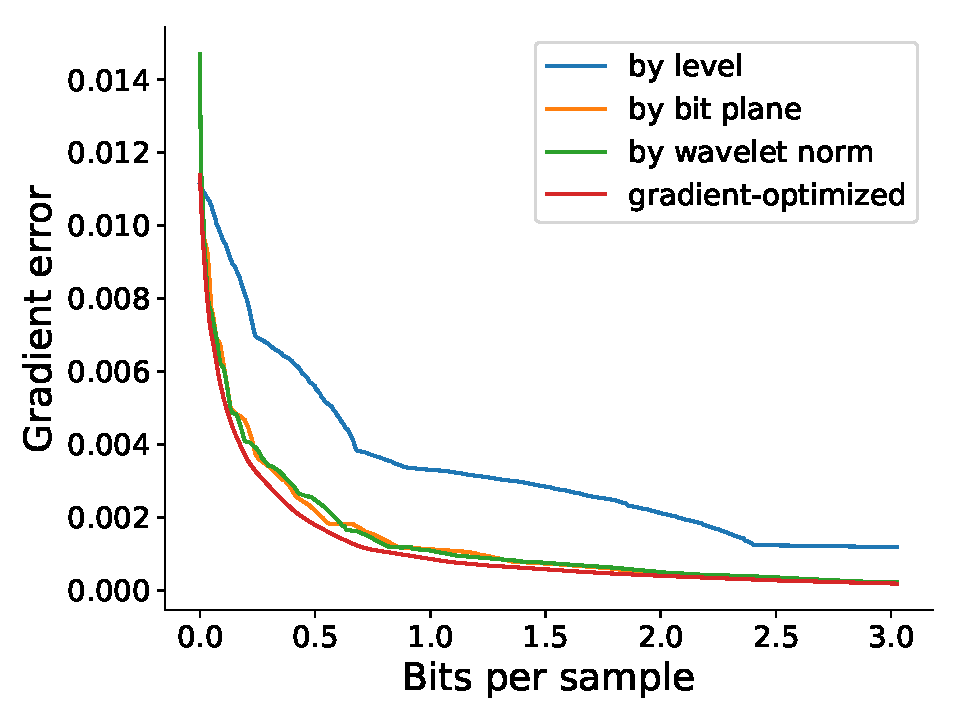
\includegraphics[width=0.24\linewidth]{gradient/gradient-optimized-diffusivity}\vspace{-0.5em}}}
\subcaptionbox{\emph{turbulence} $[0.465e{-}3, 12.19]$}{%
{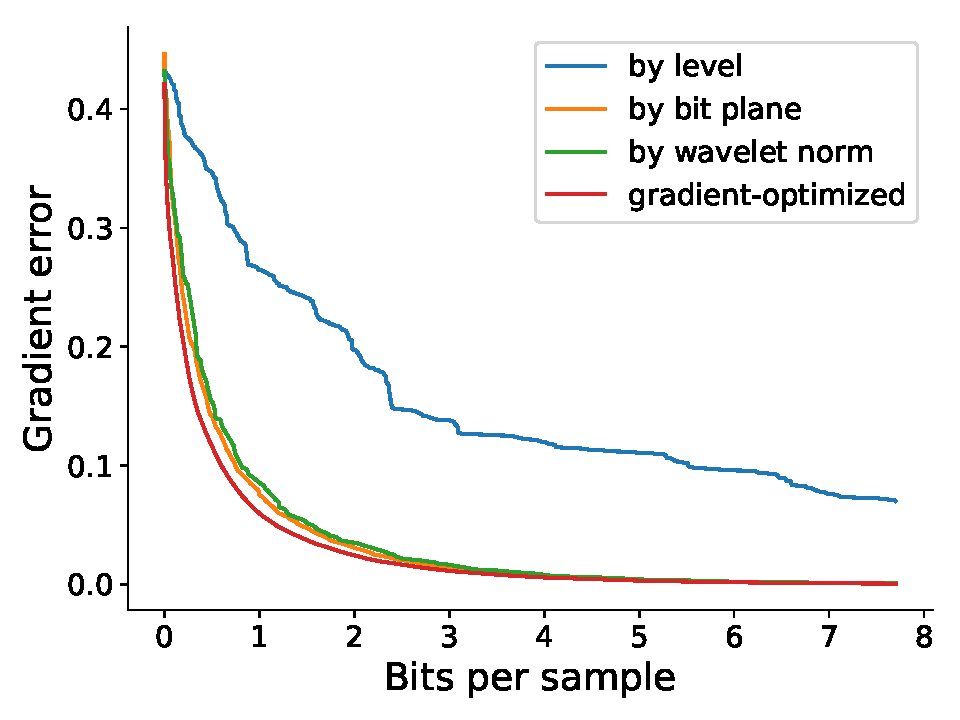
\includegraphics[width=0.24\linewidth]{gradient/gradient-optimized-turbulence}\vspace{-0.5em}}}
\subcaptionbox{\emph{pressure} $[2.542e{-}6, 0.536]$}{%
{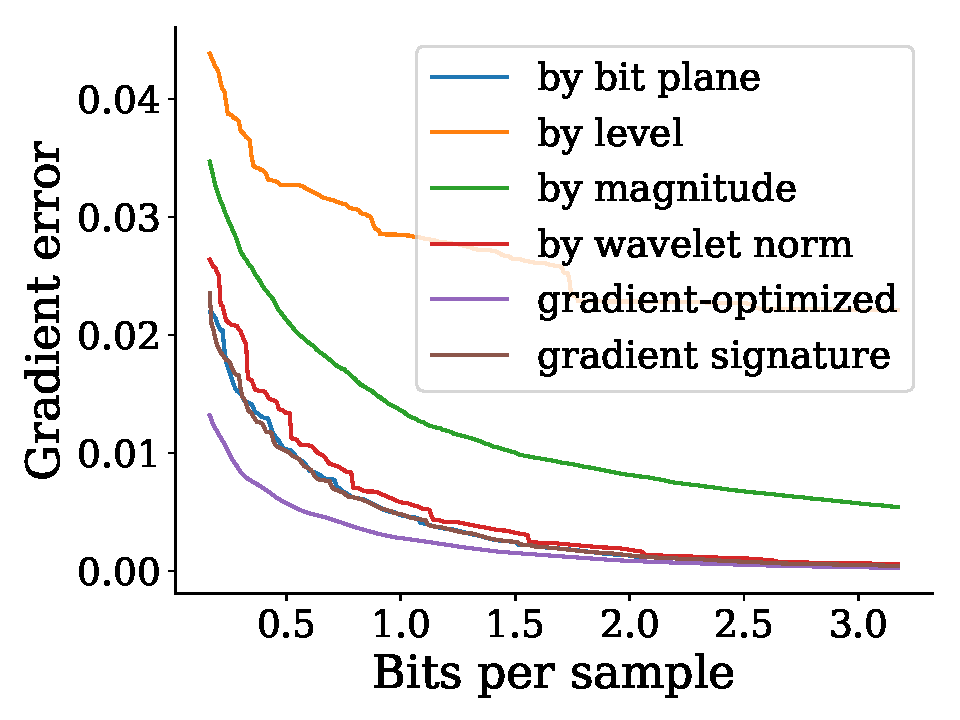
\includegraphics[width=0.24\linewidth]{gradient/gradient-optimized-pressure}\vspace{-0.5em}}} 
\vspace{-0.5em}
\caption{Gradient error of reconstructed functions. Lower gradient error is better. Leading zero
packets are removed, and the plots are truncated in the same way as in~\Cref{fig:rmse-optimized}.
The numbers in brackets are the ranges of original gradient magnitudes. The trend in error, in all
cases, is $\sgop < \sgsg \approx \sbit \approx \swav < \smag < \slvl$.}
\label{fig:gradient-error-comparison}
\vspace{1em}

\centering
\subcaptionbox{\emph{by level} (\slvl)}{%
{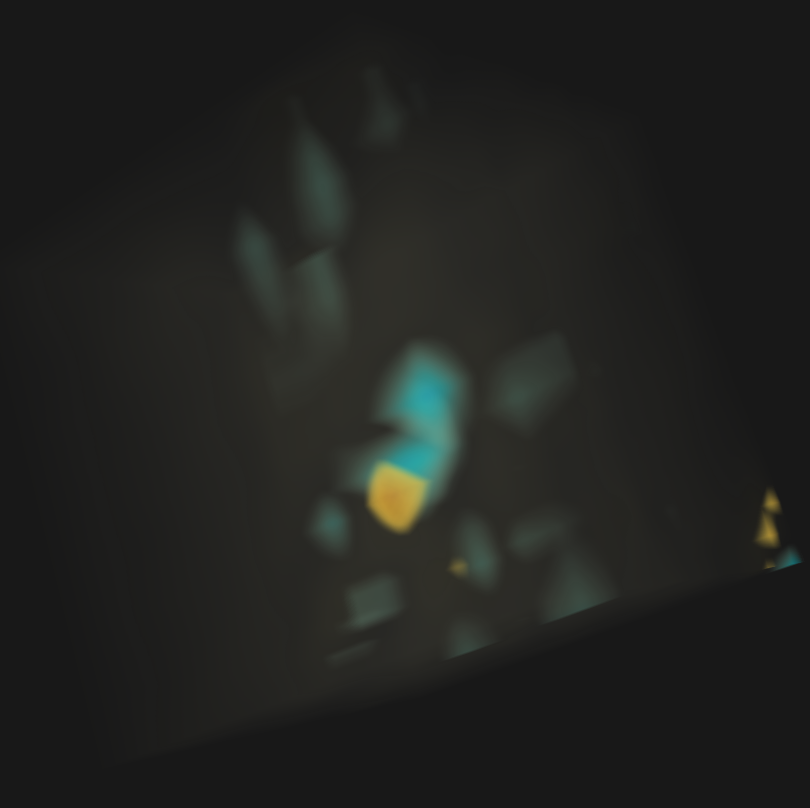
\includegraphics[width=0.16\linewidth]{gradient/gradient-turbulence-level}\vspace{-0.5em}}}
\subcaptionbox{\emph{by bit plane} (\sbit)}{%
{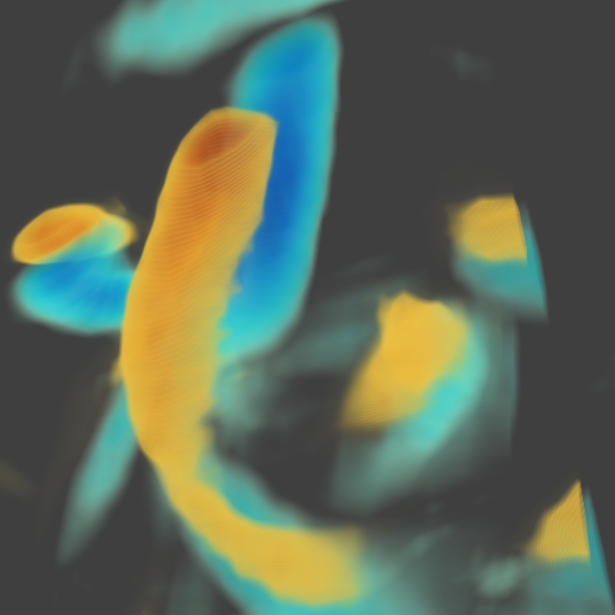
\includegraphics[width=0.16\linewidth]{gradient/gradient-turbulence-bit-plane}\vspace{-0.5em}}}
\subcaptionbox{\emph{by wavelet norm} (\swav)}{%
{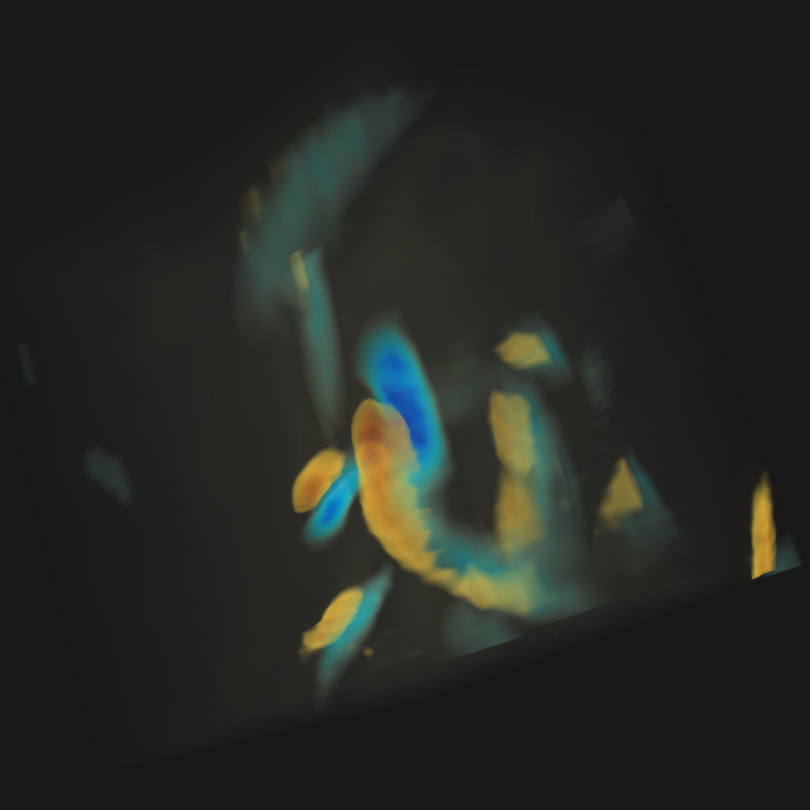
\includegraphics[width=0.16\linewidth]{gradient/gradient-turbulence-wavelet-norm}\vspace{-0.5em}}}
\subcaptionbox{\emph{by magnitude} (\smag)}{%
{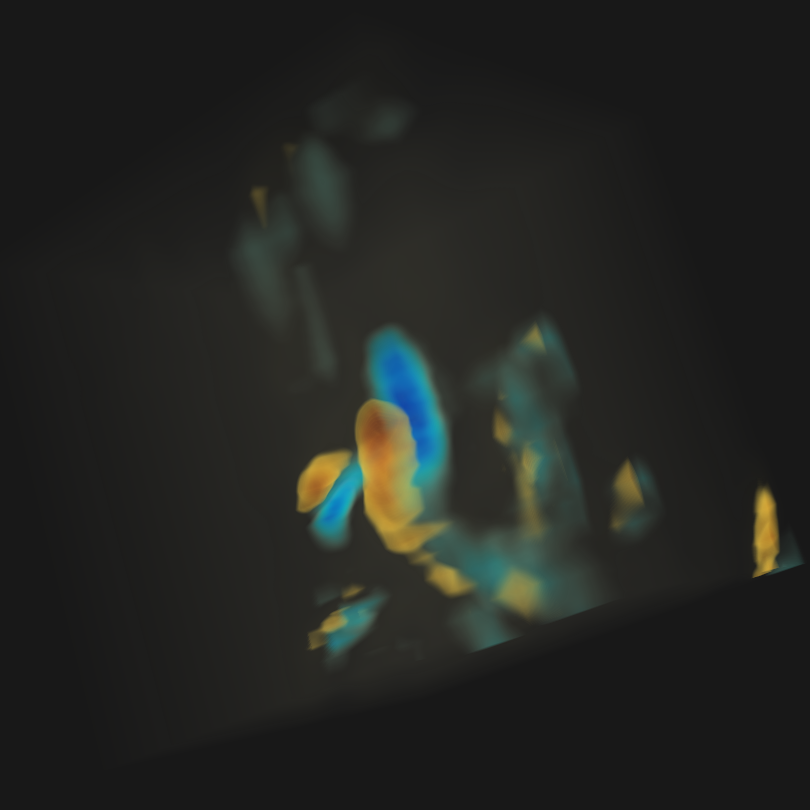
\includegraphics[width=0.16\linewidth]{gradient/gradient-turbulence-magnitude}\vspace{-0.5em}}}
\subcaptionbox{\emph{by signature} (\sgsg)}{%
{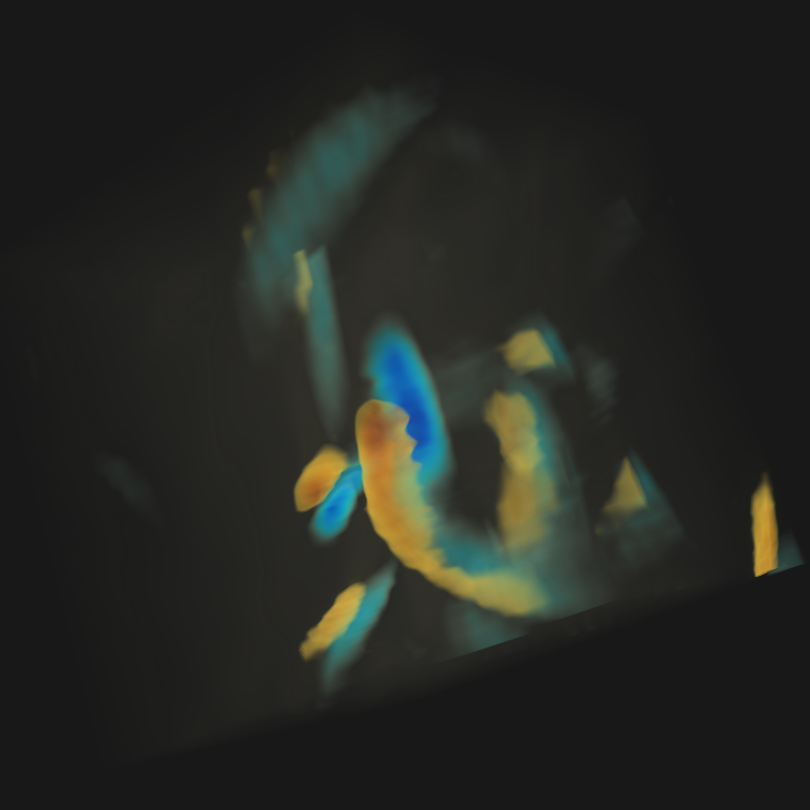
\includegraphics[width=0.16\linewidth]{gradient/gradient-turbulence-signature.png}\vspace{-0.5em}}}
\subcaptionbox{\emph{reference}}{%
{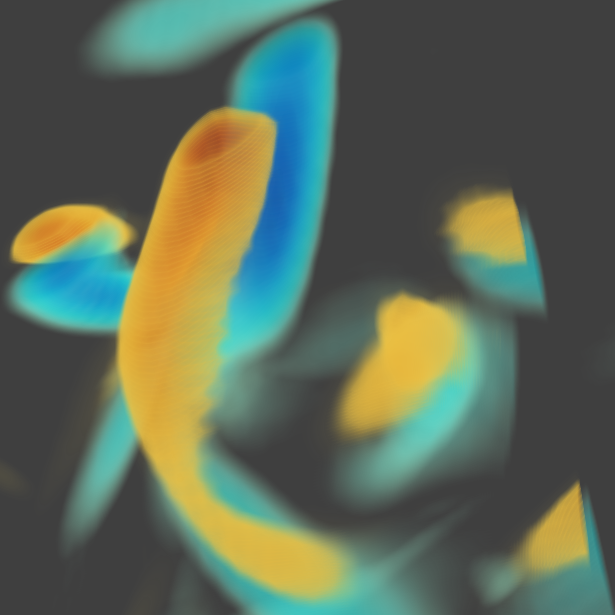
\includegraphics[width=0.16\linewidth]{gradient/gradient-turbulence-groundtruth.png}\vspace{-0.5em}}}
\vspace{-0.5em}
\caption{The $x$-component of the ($64^3$) gradient field of \emph{turbulence}, reconstructed at 0.3
bps. \sbit, \swav, and \sgsg produce visually comparable gradient fields.}
\label{fig:gradient-rendering-diff}
%\vspace{-1em}
\end{figure*}

% figure for laplacian
\begin{figure*}[!t]
\centering
\subcaptionbox{\emph{boiler} $[-0.393, 0.221]$}
{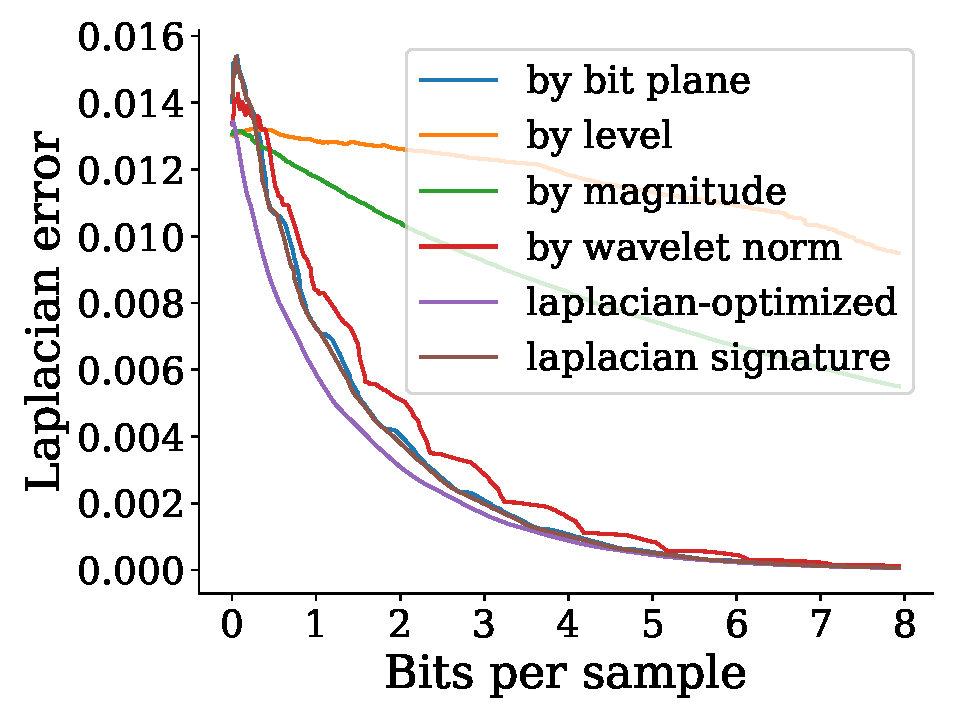
\includegraphics[width=0.24\linewidth]{laplacian/laplacian-optimized-boiler}\vspace{-0.5em}}
\subcaptionbox{\emph{diffusivity} $[-0.404, 0.269]$}
{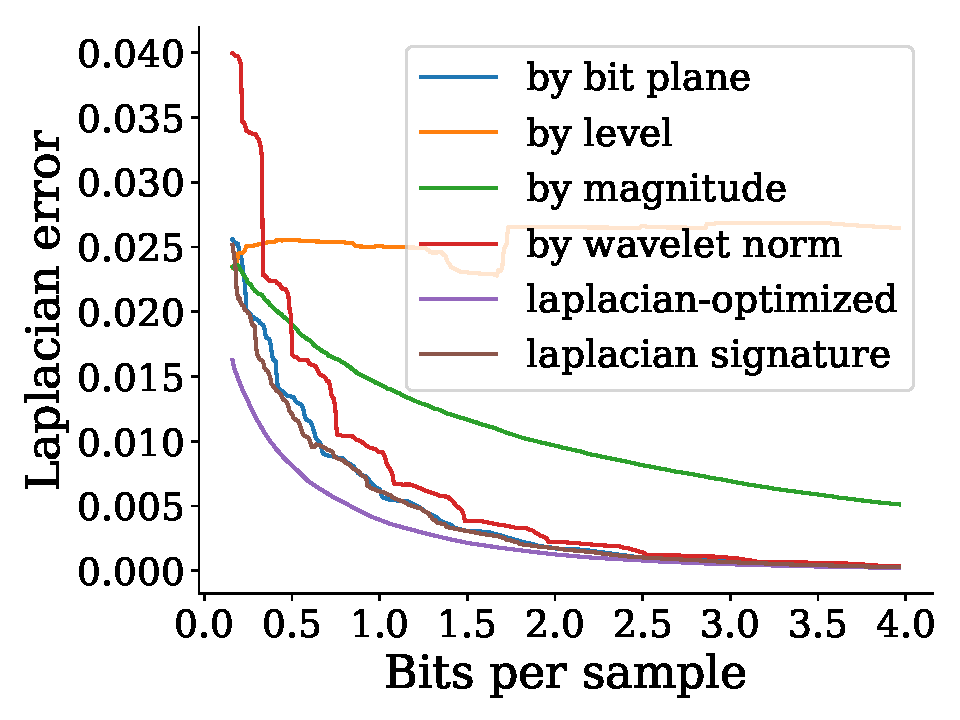
\includegraphics[width=0.24\linewidth]{laplacian/laplacian-optimized-diffusivity}\vspace{-0.5em}}
\subcaptionbox{\emph{turbulence} $[-17.44, 11.99]$}
{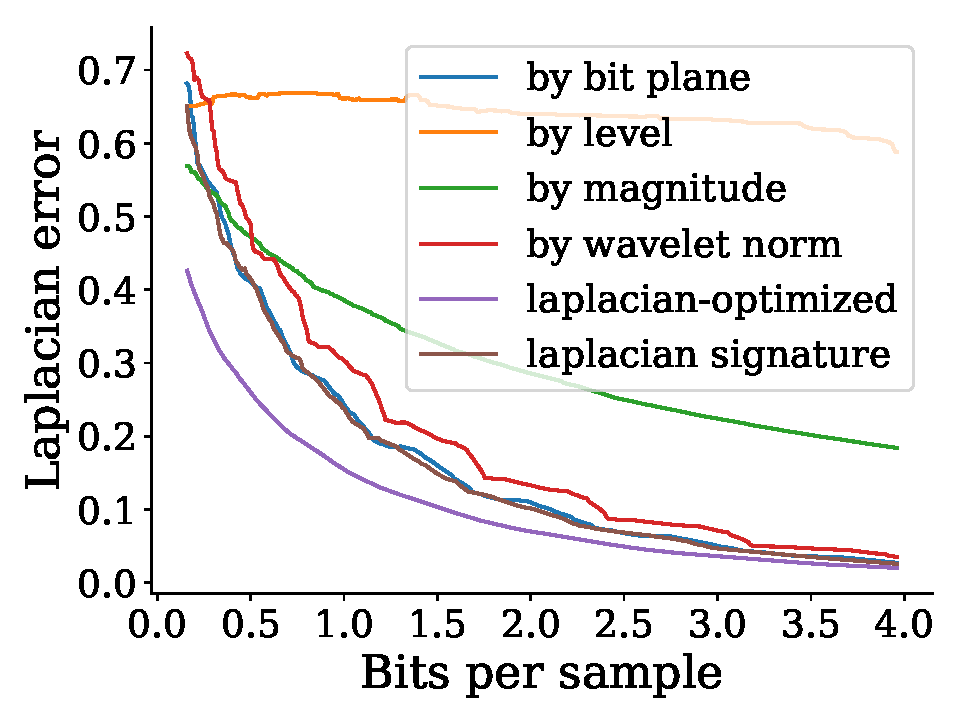
\includegraphics[width=0.24\linewidth]{laplacian/laplacian-optimized-turbulence}\vspace{-0.5em}}
\subcaptionbox{\emph{pressure} $[-0.467, 0.432]$}
{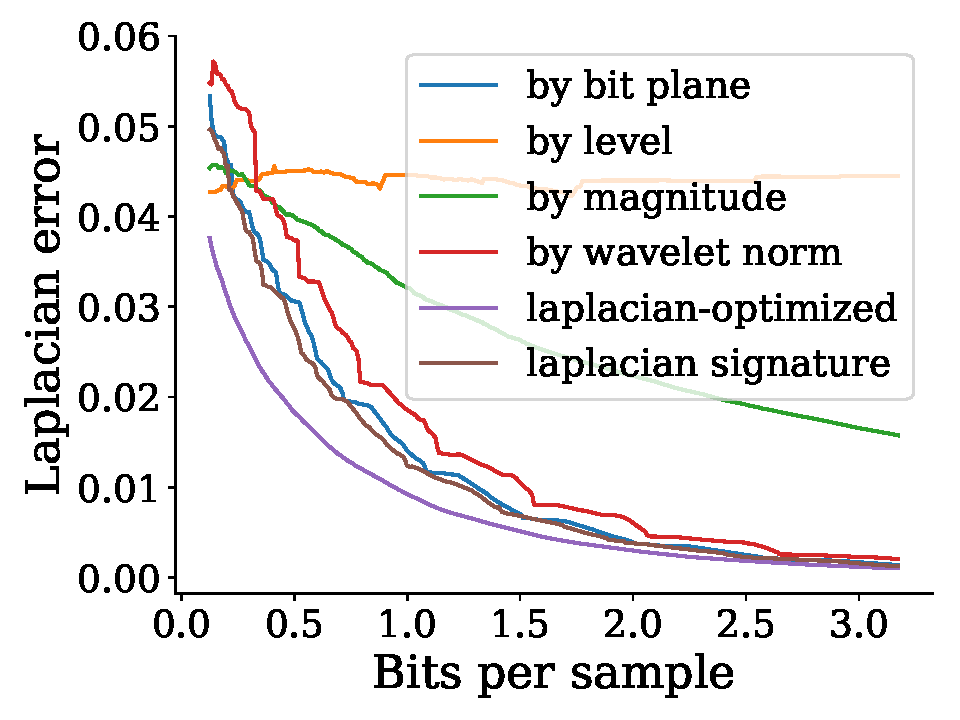
\includegraphics[width=0.24\linewidth]{laplacian/laplacian-optimized-pressure}\vspace{-0.5em}}
\vspace{-0.5em}
\caption{Laplacian error comparison among streams. The plots are truncated to better highlight
differences without discarding important information. The numbers in brackets are the ranges of the
original Laplacian fields. In all cases, in terms of error, $\slop <\slsg < \sbit < \swav < \smag <
\slvl$.}
\label{fig:laplacian-error-comparison}
\vspace{-1.5em}
\end{figure*}

\subsection{Derivative Computation} \label{sec:derivatives}

Computation of derivative-based quantities is important in data analysis. Examples include vorticity
(curl) computation from velocity fields to identify vortical structures, gradient computation for
accurate Morse segmentation and shading, and ridge extraction (e.g., for Lagrangian coherent
structures). In this paper, derivatives are always computed using finite differences, which is
common in practice. In this section, we use 32 bits for quantization to ensure enough precision for
finite differences. We always compute finite differences on the finest resolution grid to avoid
computing distances between quantities defined on grids of different resolutions.

\subsubsection{Gradient Computation} \label{sec:gradient}

Given a function $f$ defined on a grid, its gradient at a grid point \mbox{$\x = (x,y,z)$} is
$\nabla f(\x) = \left(\frac{\partial f}{\partial x}, \frac{\partial f}{\partial y}, \frac{\partial
f}{\partial z}\right)$. For accuracy, we use a five-point stencil to compute the gradient, i.e.,
$\frac{\partial f}{\partial x} \approx \frac{1}{12}f(x-2,y,z) - \frac{2}{3}f(x-1,y,z) +
\frac{2}{3}f(x+1,y,z) - \frac{1}{12}f(x+2,y,z)$, but we note that the relative performances of the
streams stay the same, using the more common two- and three-point formulas. The error between a
gradient field $\nabla f$, and its low-bit-rate approximation $\nabla f'$, is defined as
$\err(\nabla f', \nabla f) = \sqrt{\frac{1}{N} \sum_{i=1}^{N}{\norm{\nabla f'(\x_i)-\nabla
f(\x_i)}^2}}$. Using~\Cref{alg:greedy}, we compute a \emph{gradient-optimized} stream, \sgop, that
minimizes the difference between the reconstructed and the original gradient fields.

\Cref{fig:gradient-error-comparison} shows the gradient error incurred by different streams for four
data sets. In general, we observe the ordering of performance (from best to worst) as: \sgop, \sgsg,
\sbit, \swav, \smag, \slvl. This ordering can also be seen in~\Cref{fig:gradient-rendering-diff},
where the $x$-component of the gradient field for \emph{tuburlence} is rendered at 0.3 bps. Unlike
the RMSE case, \sbit performs nearly the same as \swav.

To investigate this difference, we extract a 1D line from the \emph{plasma} data set and reconstruct
the function using \sbit and \swav at 0.6 bps (\Cref{fig:bit-plane-vs-wavelet-norm-gradient}).
\swav's reconstruction is more accurate on average compared to \sbit, which captures well the
function's shape (due to the presence of fine-scale bits), but not the function values (due to the
lack of precision in the coarse-scale coefficients). Functions reconstructed with \sbit tend to be
``shifted'' in the range domain, as seen in ~\Cref{fig:bit-plane-vs-wavelet-norm-gradient}. However,
the gradient operator has the tendency to cancel the shifting effect, bringing the performance of
\sbit closer to that of \swav.

\sgop again outperforms the rest of the streams. \slvl and \smag perform poorly for gradient
computation, lacking the resolution to capture sharp features. \sgsg mostly closely follows \sbit in
performance but outperforms it for \emph{boiler}. Again, compared to the other fields, \emph{boiler}
is less smooth, resulting in less spatial coherency in the magnitudes of the fine-scale
coefficients, which \sgop and \sgsg can take advantage of, whereas \swav or \sbit do not take into
account actual bit values. Overall, the results suggest that besides minimizing RMSE, \swav also
works well for gradient computation, although for the latter task, \sbit is also good alternative.

\subsubsection{Laplacian Computation}\label{sec:laplacian}

The Laplace operator is a second-order differential operator defined as the divergence of the
gradient field. The Laplacian of a 3D field is defined as $\Delta f = 
\frac{{\partial}^2}{\partial{x^2}}f+\frac{{\partial}^2}{\partial{y^2}}f+\frac{{\partial}^2}{\partial{z^2}}f$.
%
Using a five-point finite difference, we approximate 
%$\frac{{\partial}^2}{\partial{x^2}}f(x,y,z)
$\frac{{\partial}^2 f}{\partial{x^2}}
\approx
-\frac{1}{12}f(x-2,y,z)+\frac{4}{3}f(x-1,y,z)-\frac{5}{2}f(x,y,z)+\frac{4}{3}f(x+1,y,z)-\frac{1}{12}f(x+2,y,z)$.
We use the root-mean-square error to compare two Laplacian fields, i.e., $\err(\Delta f',\Delta
f)=\text{RMSE}(\Delta f',\Delta f)$. We use~\Cref{alg:greedy} to compute a
\emph{Laplacian-optimized} stream, \slop, which minimizes $\err$, and an \slsg stream from its
signature.~\Cref{fig:laplacian-error-comparison} plots the errors for all relevant streams. The
plots here largely follow the ones in~\Cref{fig:gradient-error-comparison}, in terms of relative
performance among the streams, but with more discernible gaps between \sbit and \slsg, as well as
between \slsg and \sbit. The results suggest that similar to the gradient case, computation of the
Laplacian favors resolution over precision, but to a higher degree.